\begin{frame}{Dynamic Binding}
    \begin{itemize}
        \item When designing a system you usually know which kind of interface
            do you want but not the concrete implementation

        \vspace{5mm}

        \item The goal is to reduce the effort in changing implementations

        \vspace{5mm}

        \item \textbf{Dynamic Binding:} The address of the code in a function
            invocation is determined at the last possible moment: based 
            on the dynamic type of the object at runtime
    \end{itemize}
\end{frame}

\begin{frame}{Virtual Functions}
    \begin{center}
        \begin{tikzpicture}[]
            \node[] at (0mm,0mm){
                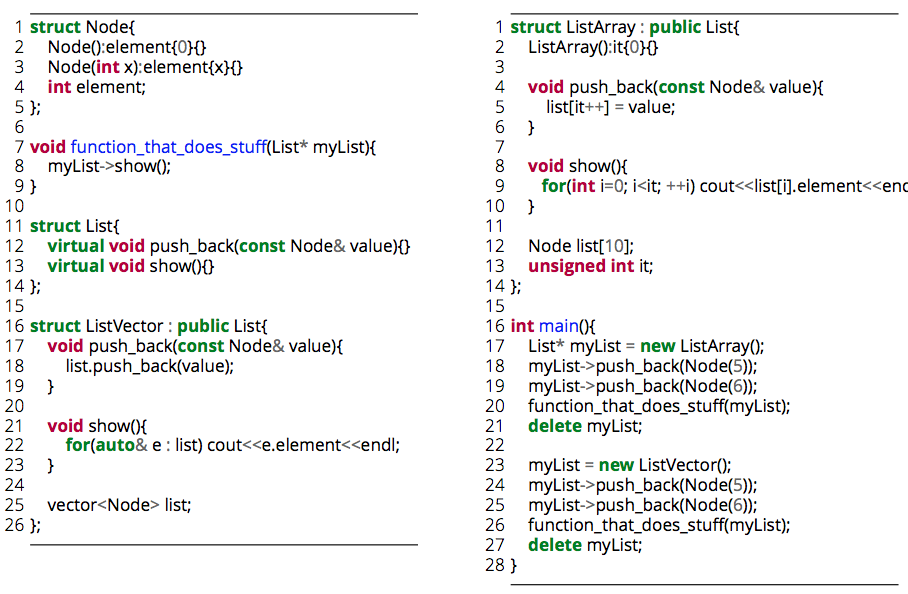
\includegraphics[height=70mm]{/home/elf/PersonalProjects/MetaTalk/figures/ddp1.png}\hspace{5mm}
            };
        \end{tikzpicture}
    \end{center}
\end{frame}

\begin{frame}{Virtual Functions}
    \begin{center}
        \begin{tikzpicture}[]
            \node[] at (0mm,0mm){
                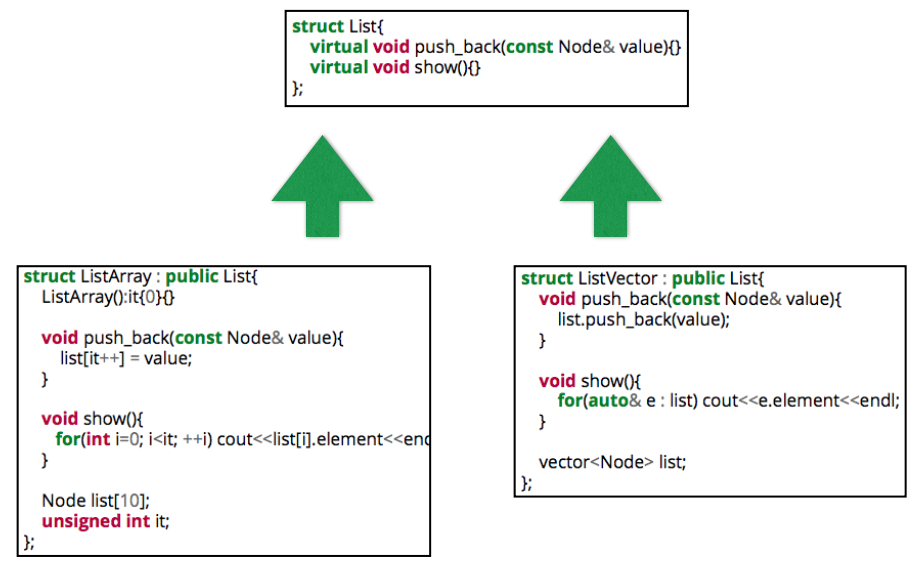
\includegraphics[height=70mm]{/home/elf/PersonalProjects/MetaTalk/figures/classdiag.png}\hspace{5mm}
            };
        \end{tikzpicture}
    \end{center}
\end{frame}


